\documentclass[MoviesApp.tex]{subfiles}

\begin{document}

\section{Movie Application}

For this part of the project we were asked to implement a simple movie lookup application from an XML database. Figure \ref{fig:movieapp} below shows a screenshot of the movie application running on the eXist environment on the local machine. The application was written in the eXist IDE environment and all the code for this application can be found on GitHub link.

\begin{figure}[H]
	\centering
	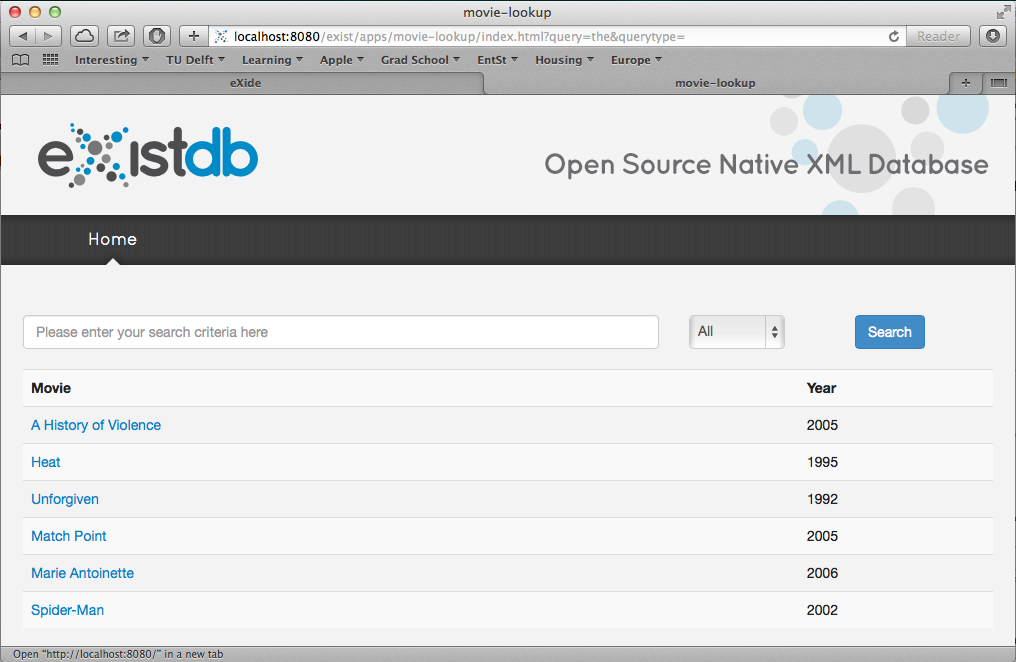
\includegraphics[width=1\textwidth]{./Figures/MovieApp.png}
	\caption{Movie Application}
	\label{fig:movieapp}
\end{figure}

\subsection{Search Criteria}
The search bar allows users to search movies with the following options:

\begin{itemize}
\item Title
\item Keywords
\item Year
\item Director
\item Actor
\item Genre
\end{itemize}

\subsection{Selecting Movie From Returned Results}
If matching movies are found, a list is returned showing the movie title and release year. More details about the movie can be found by clicking on the movie title as shown in Figure \ref{fig:movieappselected}.

\begin{figure} [H]
	\centering
	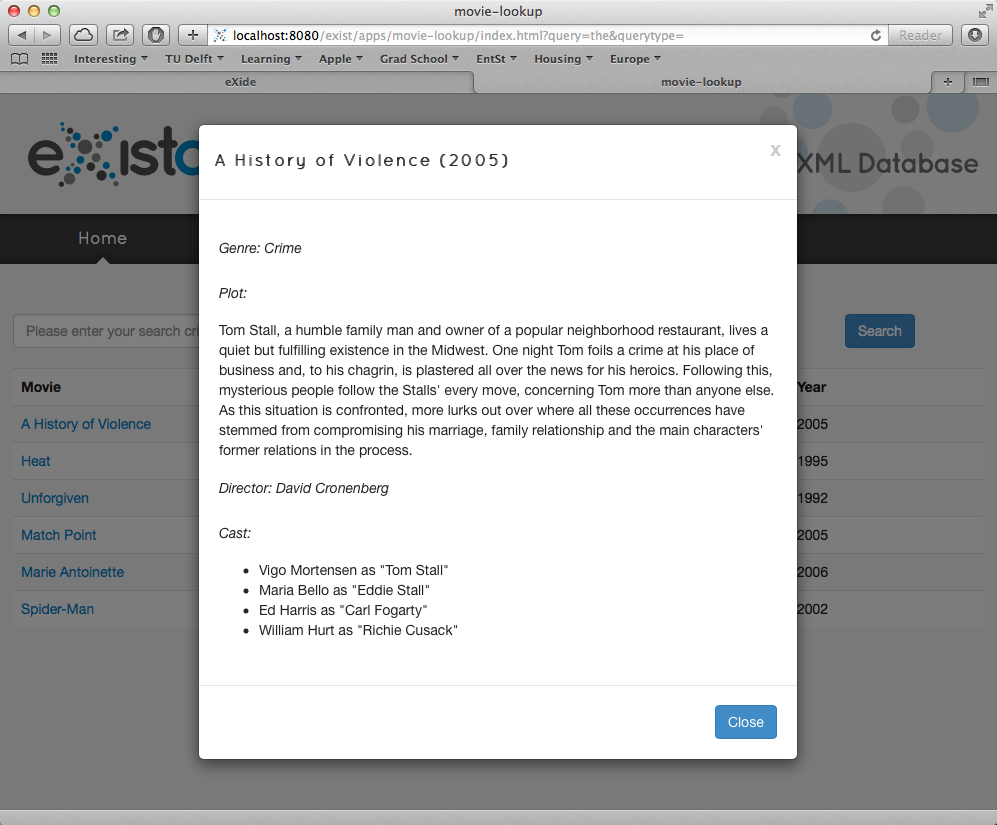
\includegraphics[width=1\textwidth]{./Figures/MovieAppSelected.png}
	\caption{Additional Movie Information}
	\label{fig:movieappselected}
\end{figure}

\end{document}